\documentclass[10pt]{article}
\usepackage[latin1]{inputenc}
\usepackage{geometry}                % See geometry.pdf to learn the layout options. There are lots.
\geometry{letterpaper}				% Activate for for rotated page geometry
%\geometry{landscape} 
%\usepackage[parfill]{parskip}		% Activate to begin paragraphs with an empty line rather than an indent
\usepackage{graphicx}
\usepackage{epstopdf}
\usepackage{mathptmx}
\usepackage{mathtools}
\usepackage{float}
\usepackage{dblfloatfix}
\usepackage{amsmath}
\usepackage{amsfonts}
\usepackage{amssymb}
\usepackage{multicol}
\usepackage{wrapfig}
\usepackage{amsmath}
\DeclareGraphicsRule{.tif}{png}{.png}{`convert #1 `dirname #1`/`basename #1 .tif`.png}

\begin{document}
\title{Upper Atmosphere and Ionosphere Assignment 4}
\author{Jonathan Nickerson}
\date{April 1, 2012}
\maketitle

\section{Introduction}
In this assignment I added gradients in the O+ density, advection to the O+ density and added electron temperature. Additionally I added the ion loss processes from tabel 8.4 and 8.5. I did not realize that we needed these on the last homework. Adding these losses did change the numbers slightly but not significantly. For the vertical advection I varied the velocity. I started with -200 m/s and allowed the velocity to vary between -200m/s and +200m/s to investigate how different velocities, both positive and negative will affect the behavior of the O+. Below are the plots that were output by my code with some brief explanations.

\begin{figure}[H]
	\centering
		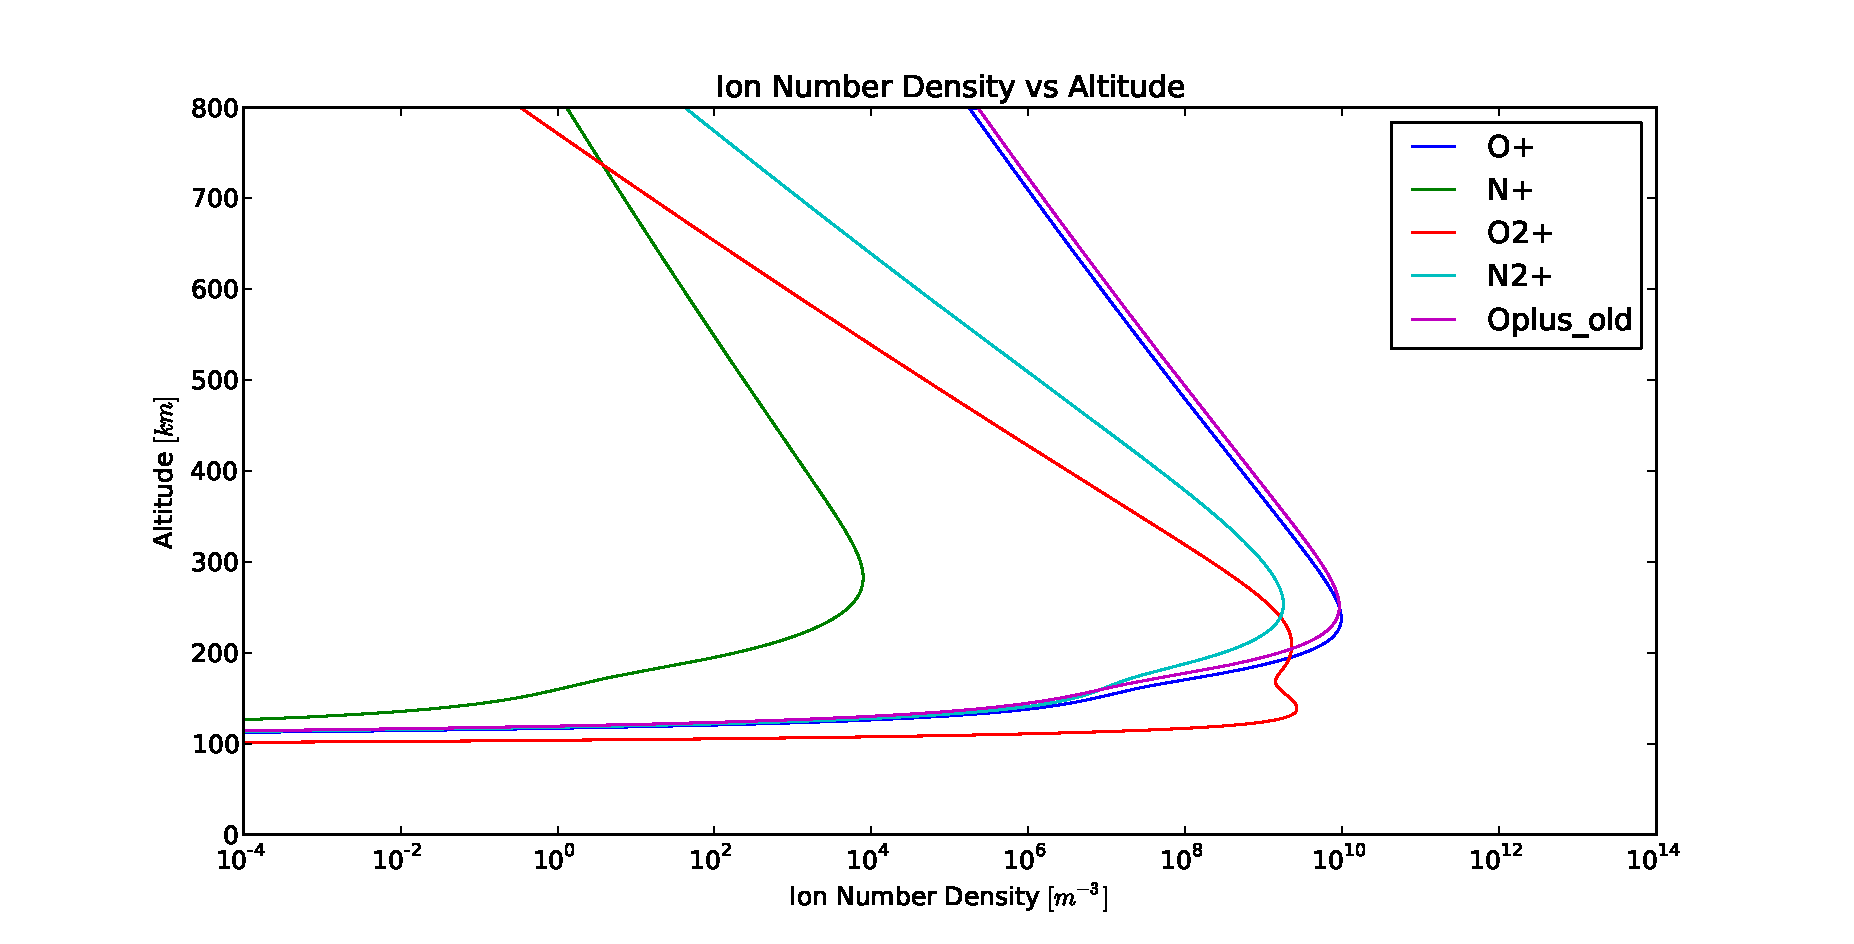
\includegraphics[width=0.99\textwidth]{./figures/B/use/Ion_Number_Density_vs_Altitude_100_800_-200.eps}
	\caption{This is a plot of ion number density vs altitude for zenith angle $-\frac{\pi}{2}$ (dawn) after 1 day. With advection velocity of -200 m/s. After 1 day.}
	\label{fig:n1}
\end{figure}
\begin{figure}[H]
	\centering
		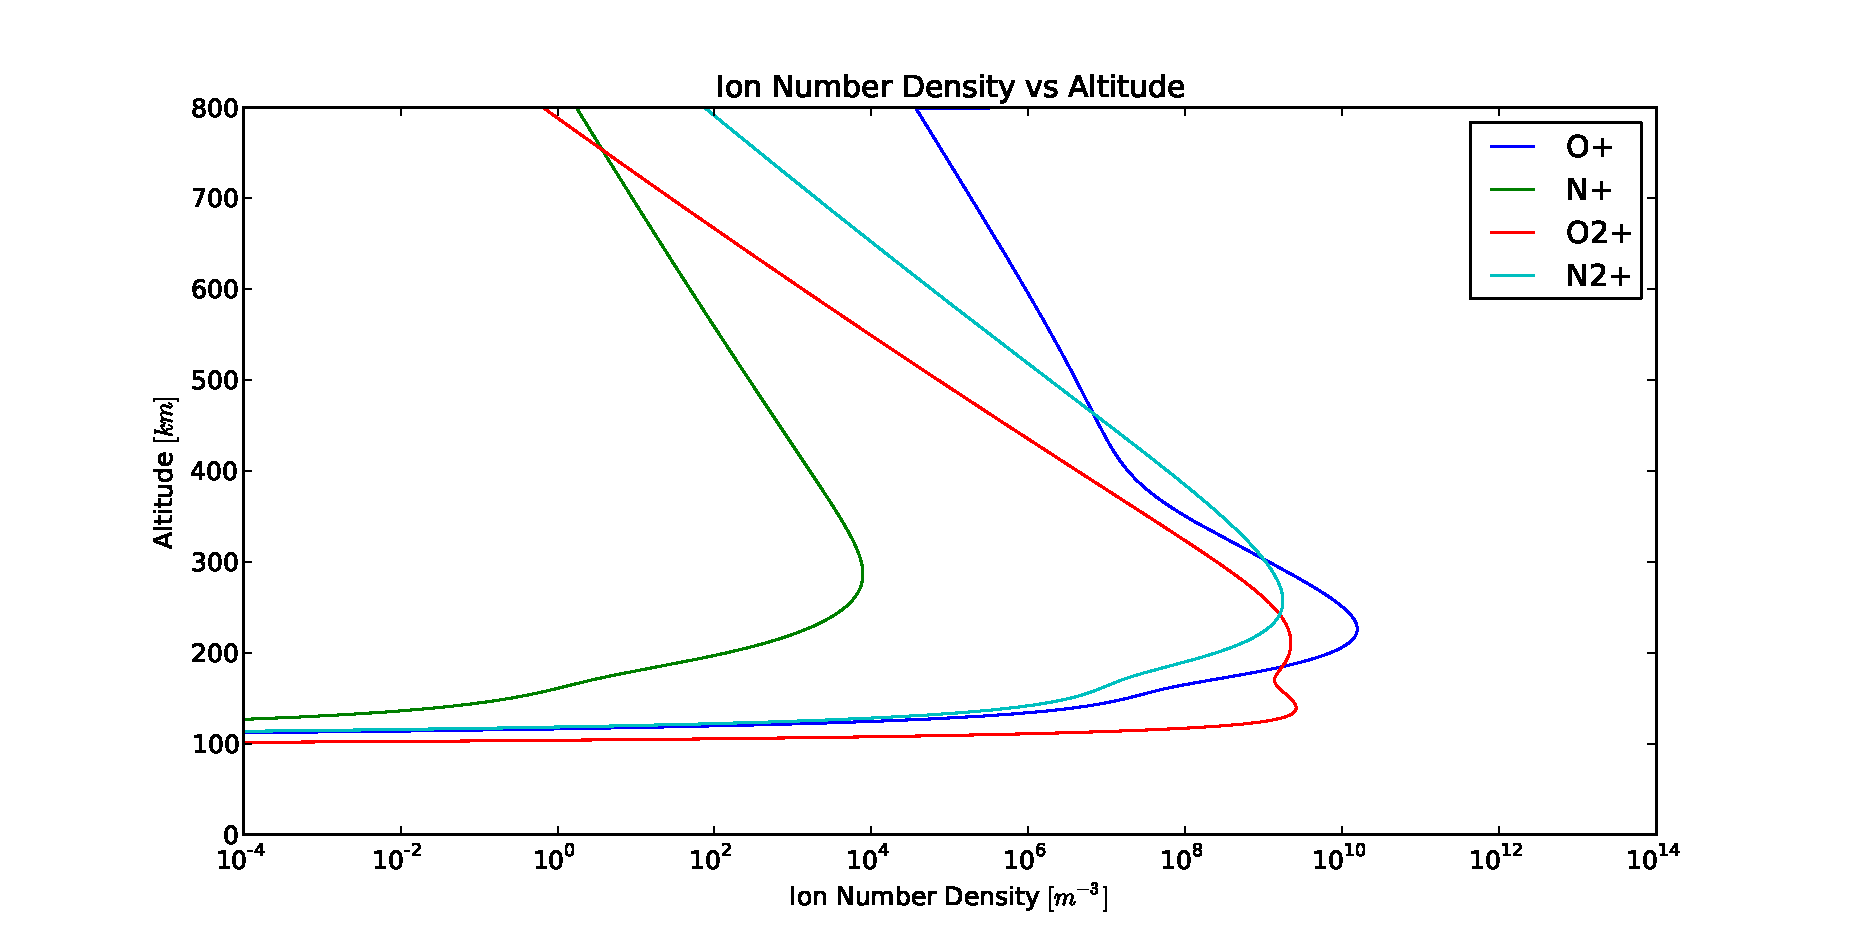
\includegraphics[width=0.99\textwidth]{./figures/B/use/Ion_Number_Density_vs_Altitude_100_800_-800.eps}
	\caption{This is a plot of ion number density vs altitude for zenith angle $-\frac{\pi}{2}$ (dawn) after 1 day. With advection velocity of -800 m/s.}
	\label{fig:n2}
\end{figure}
\begin{figure}[H]
	\centering
		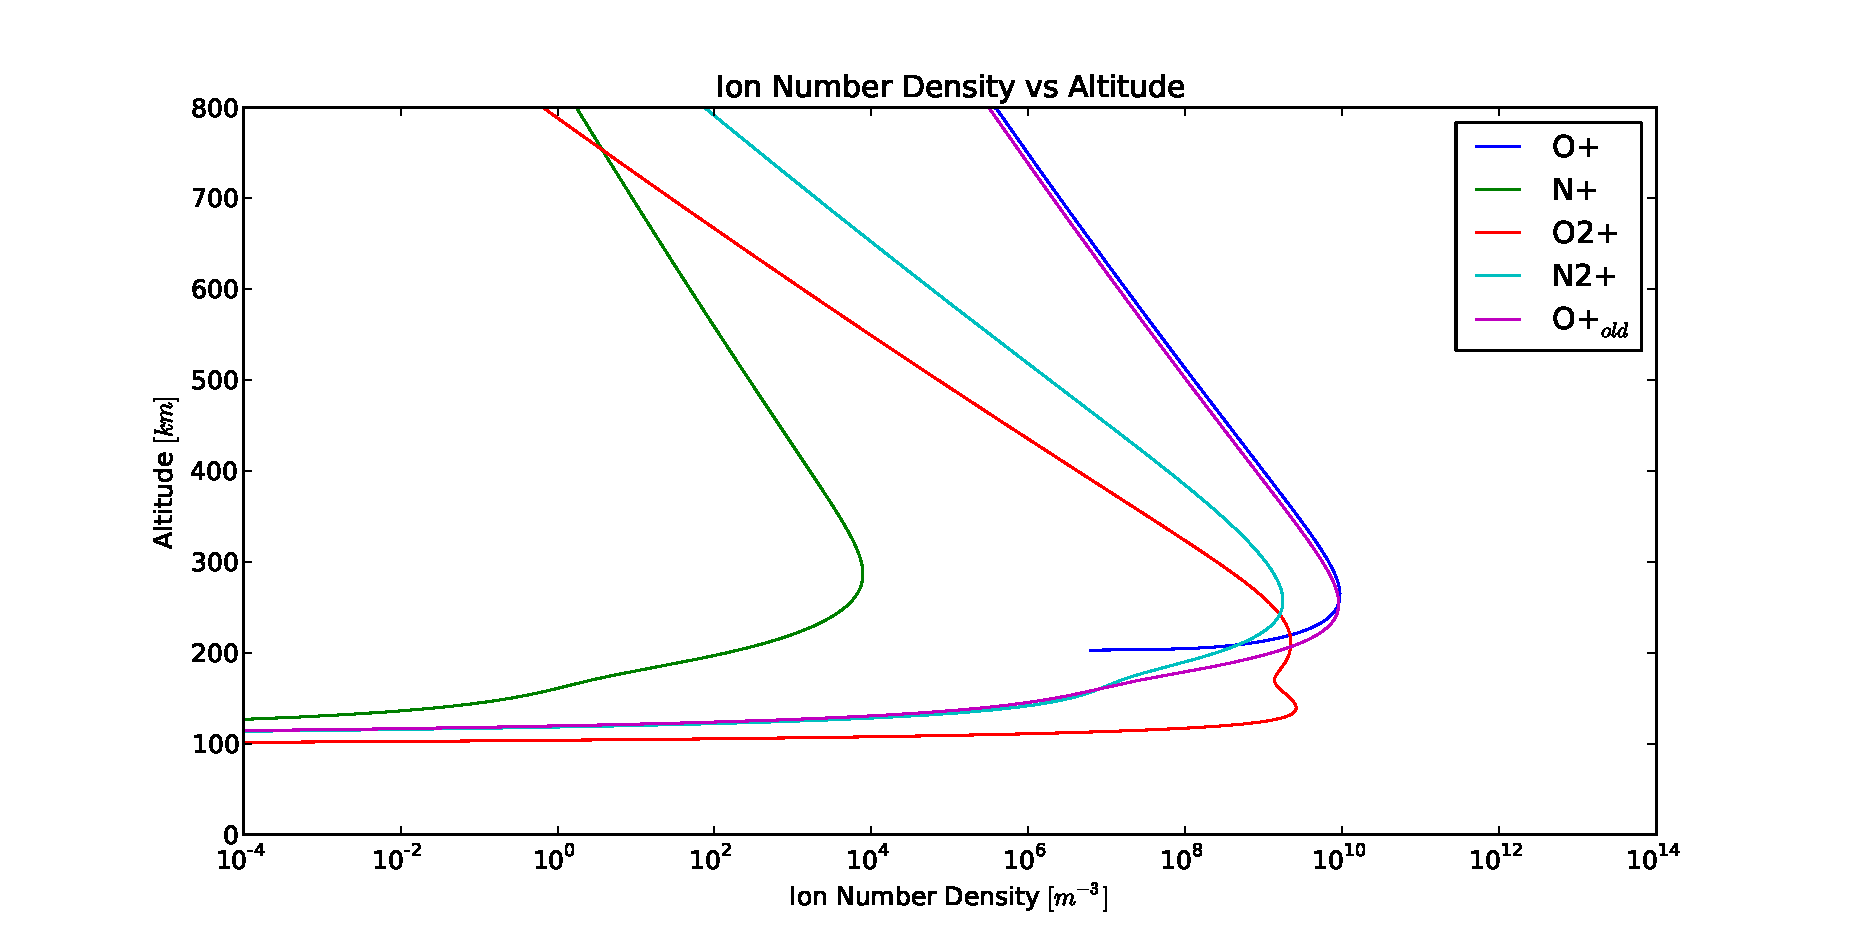
\includegraphics[width=0.99\textwidth]{./figures/B/use/Ion_Number_Density_vs_Altitude_100_800_+200.eps}
	\caption{This is a plot of ion number density vs altitude for zenith angle $-\frac{\pi}{2}$ (dawn) after 1 day. With advection velocity of +200 m/s.}
	\label{fig:n3}
\end{figure}
\begin{figure}[H]
	\centering
		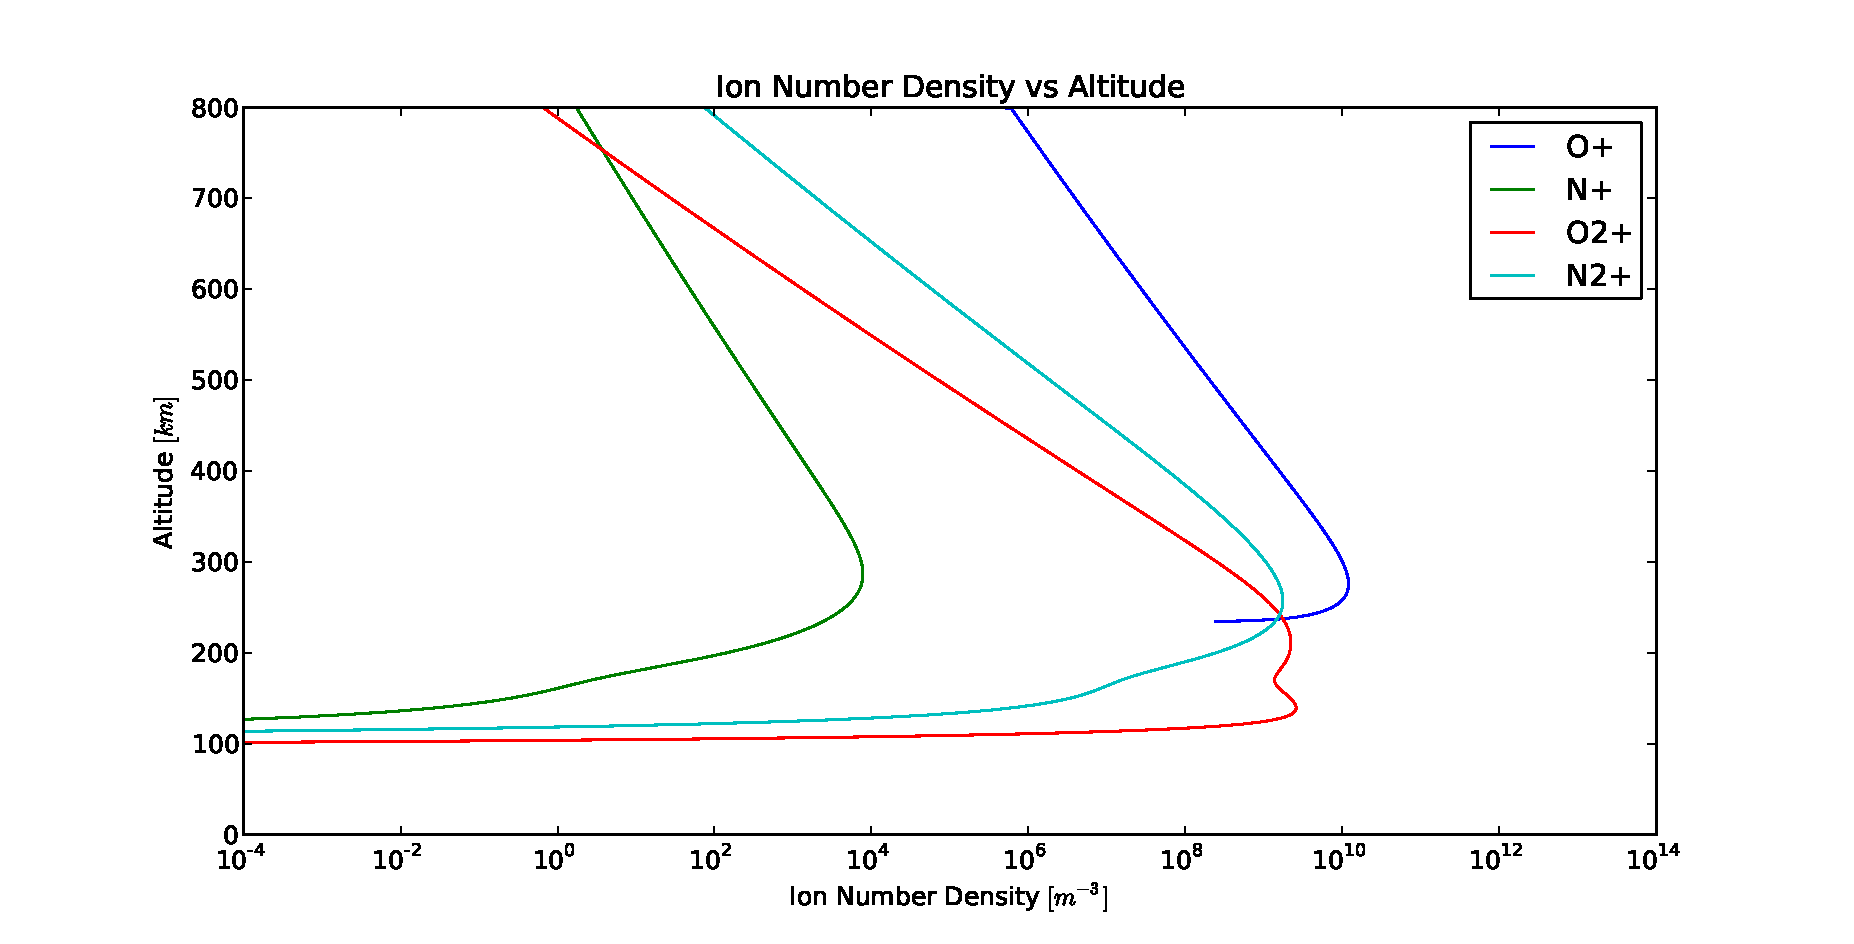
\includegraphics[width=0.99\textwidth]{./figures/B/use/Ion_Number_Density_vs_Altitude_100_800_+800.eps}
	\caption{This is a plot of ion number density vs altitude for zenith angle $-\frac{\pi}{2}$ (dawn) after 1 day. With advection velocity of +800 m/s.}
	\label{fig:n4}
\end{figure}
\begin{figure}[H]
	\centering
		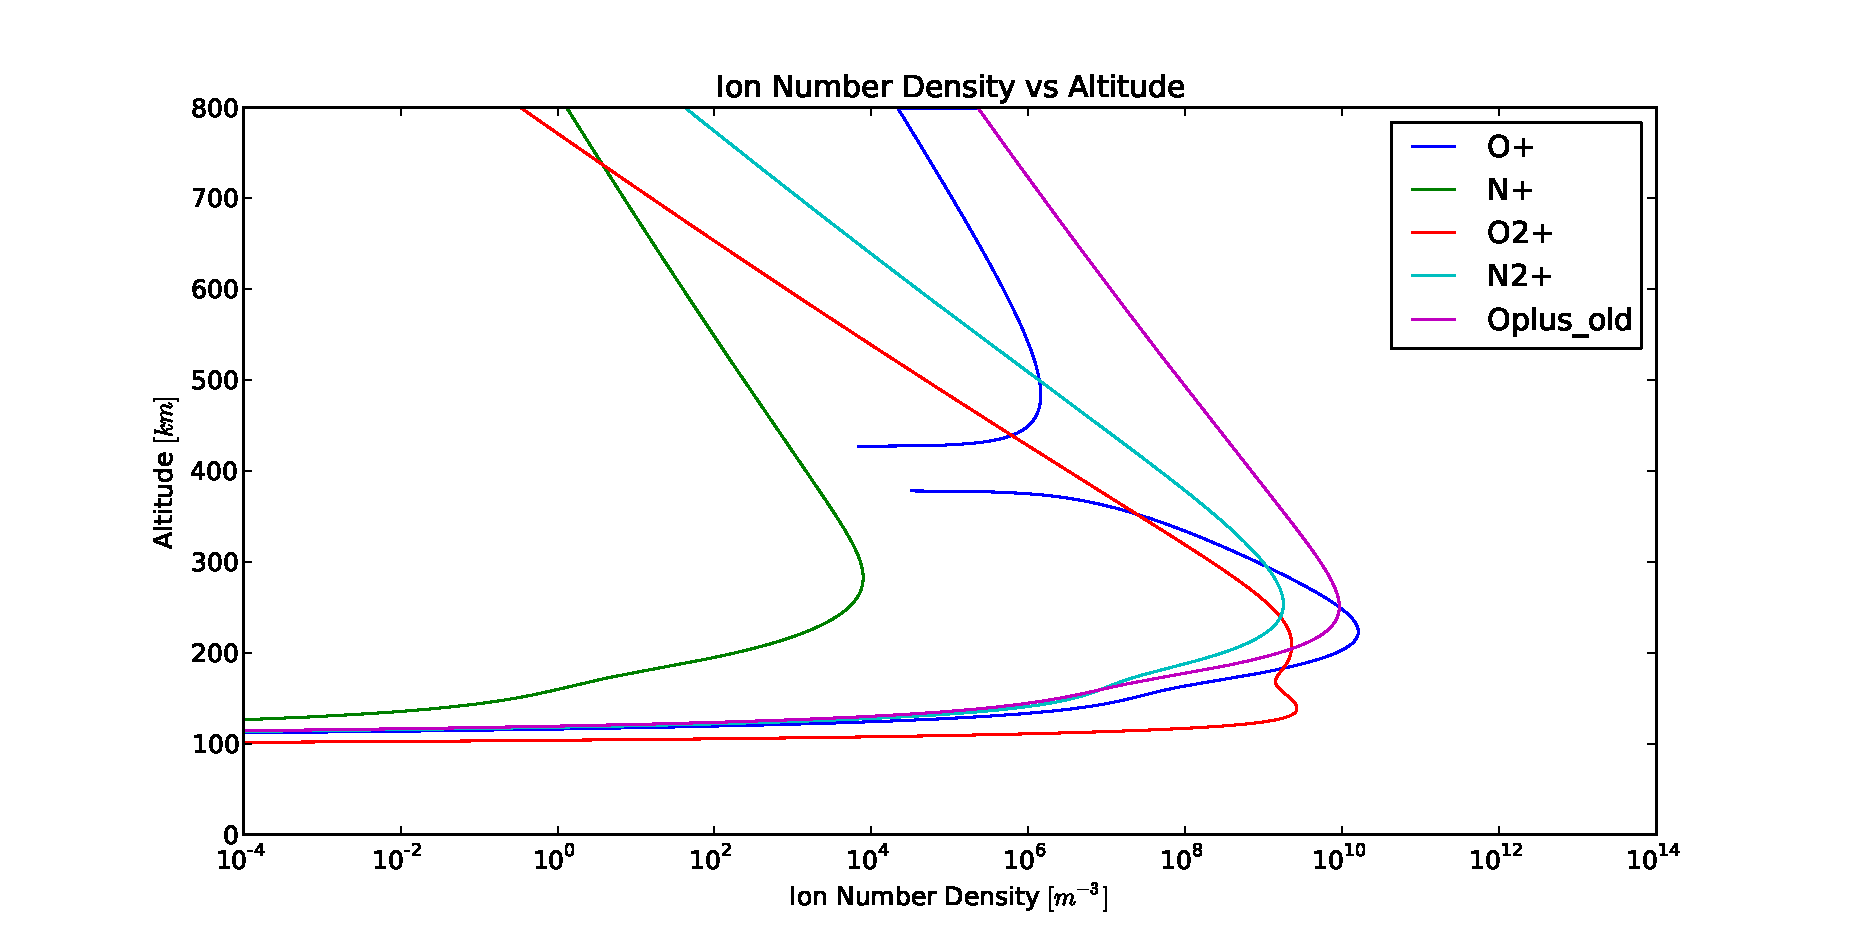
\includegraphics[width=0.99\textwidth]{./figures/B/use/Ion_Number_Density_vs_Altitude_100_800_-800_5days.eps}
	\caption{I found that if I run the code for long periods of time then the number density would become discontinuous when the wind velocity was set above $\pm$200 m/s. This is a plot of ion number density vs altitude for zenith angle $-\frac{\pi}{2}$ (dawn) after 5 days. With advection velocity of -800 m/s as before.}
	\label{fig:n4}
\end{figure}
\begin{figure}[H]
	\centering
		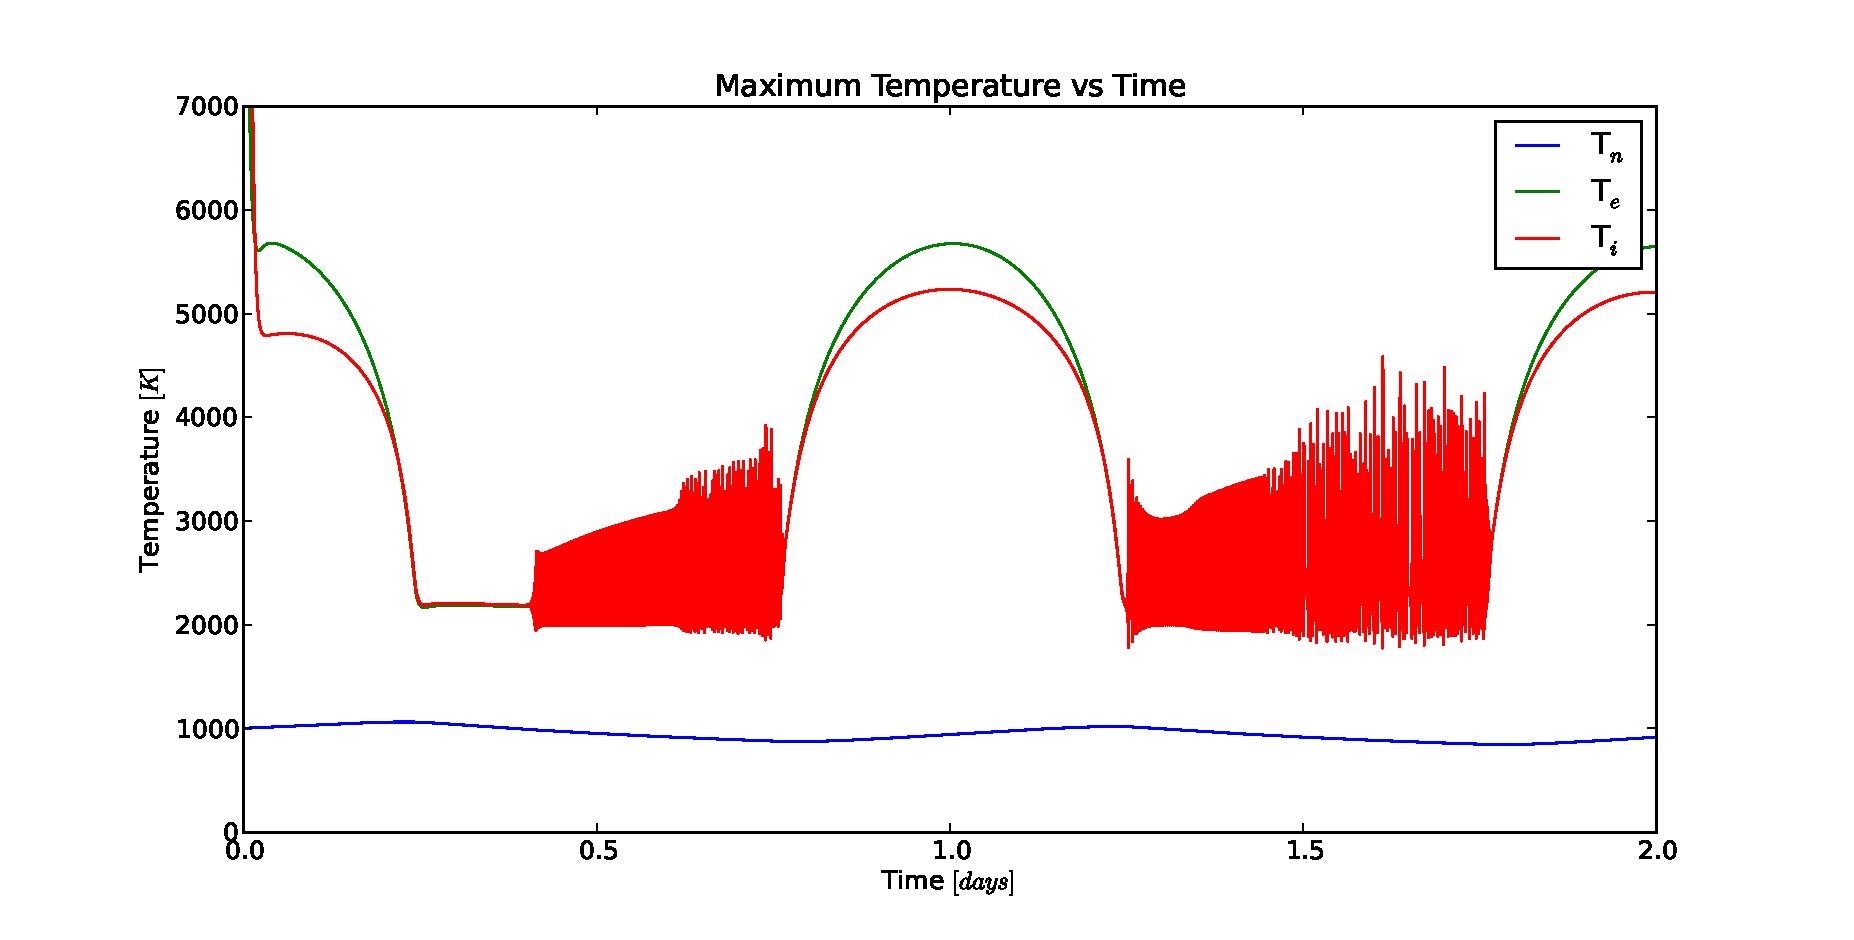
\includegraphics[width=0.99\textwidth]{./figures/B/use/T_max_vs_time.eps}
	\caption{This is a plot of maximum temperature vs time. Included is the temperature for electrons and neutrals. It runs for 5 days. The neutral temperature is the same as was shows in the last assignment. The electron temperatue behaves quite differently. First note that the electron temperature peaks at about 6000K. This is very hot compared to the neutrals. Also note that the electron temperatures respond almost excatly with the solar zenith angle. In other words the peak is exactly at noon. They reach minimum the moment the sun sets and stay at minimum until the sun comes back up. Electrons seem to heat/cool nearly instantly.}
	\label{fig:Tmax}
\end{figure}

\end{document}